\documentclass{article}
% Packages
\usepackage{amsmath}
\usepackage{amssymb}
\usepackage{graphicx}
\usepackage{booktabs}
\usepackage{algorithmic}
\usepackage{algorithm}
\usepackage{array}
\usepackage[left=2cm,right=2cm,top=2cm,bottom=2cm]{geometry}

\title{Assignment 1 - Data Mining for Networks}
\author{Correia Ambre - Jeannes Théo}
\date{January $09^{th}$, 2024}
\begin{document}
    \maketitle


    \section{Assignement 1}\label{sec:assignement-1}

    \subsection{Exercice 1}\label{subsec:exercice-1}
    1. The derivative of $f(x) = 2x^4 - 4x^3 + 3x^2 + 4x - 3$ is $f'(x) = 8x^3 - 12x^2 + 6x + 4$. \\ \\
    2. The algorithm to do the gradient descent is with $\alpha = 1/10$ is:\\
    \begin{algorithm}
        \caption{Gradient Descent}\label{alg:algorithm}
        \begin{algorithmic}
            \STATE $x := x_0$
            \WHILE{$|8x^3 - 12x^2 + 6x + 4| > \epsilon$}
            \STATE $x := x - 0.1 * (8x^3 - 12x^2 + 6x + 4)$
            \ENDWHILE
            \RETURN $x$
        \end{algorithmic}
    \end{algorithm} \\
    3. If we apply the algorithm starting from 0, we get to $-0.4$ first and end at $-0.317$.
    If we do the same algorithm starting from 10, we get $-676.4$ and then $248120326.787$. \\ \\
    4. The first gradient descend algorithm seems to converge to the minimum of the function, while the second one is clearly diverging.
    The learning rate is probably too high, and would need to be decreased to get optimal results.

    \subsection{Exercice 2}\label{subsec:exercice-2}

    3. The stochastic gradient is trained on one sample in each epoch.
    This is very unstable, and doesn't give results here.
    This could be improved by adjusting the learning rate with an optimizer such as Adam.
    The mini-batch gradient descent is trained on a small batch of samples in each epoch.
    It is more stable than the stochastic gradient descent, but less stable than the batch gradient descent.
    It converges really fast, but tends to over fit on some batches, resulting in a very unstable loss and an
    approximation of the real function that is not as good as the batch gradient descent or the stochastic gradient descent. \\ \\
    4. The non-simultaneous gradient descent seems to converge faster than the simultaneous update.
    However, they both converge to the same result, and are both very similar. \\


    \section{Assignement 2}

    \subsection{Exercice 1}

    We can do a algorithm that builds a supergraph, where each node is a graph, and each edge is the cost between two graphs.
    Using this algorithm, we can then apply a pathfinding algorithm, here a dijkstra to find the shortest path between the two graphs. Doing this, we can find the cost of the edit distance between the two graphs.  \\
    \\
    To do this efficiently, we can use heuristics to build the supergraph.
    First, there is no point in building any path that has a cost longer than the cost find with a naive algorithm.
    We can also be sure we will need to remove or add nodes when the number of nodes between graph is different.
    This means that we can do that as soon as we can, at the beginning of the algorithm for adding nodes, and when there is an isolated node for deleting nodes. \\
    We can also sort edges in 3 groups : edges that are in both graphs, edges that have one node in common, and edges that are not in common.
    This way, we can remove edges that are not in common, and then add or edit edges that have one common node in different paths. \\

    \subsection{Exercice 2}

    The table describing features values for the ideal graph kernel is :

    \begin{table}
        \centering
        \begin{tabular}{|>{\centering\arraybackslash}m{1.5cm}|>{\centering\arraybackslash}m{1cm}|>{\centering\arraybackslash}m{1cm}|>{\centering\arraybackslash}m{1cm}|>{\centering\arraybackslash}m{1cm}|}

            \toprule
            \textbf{}                                                        & 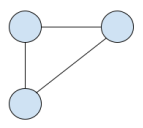
\includegraphics[width=1cm,keepaspectratio]{images/triSujet} & 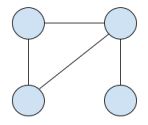
\includegraphics[width=1cm,keepaspectratio]{images/tri+Sujet} & 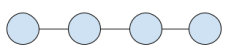
\includegraphics[width=1cm,keepaspectratio]{images/ligneSujet} & 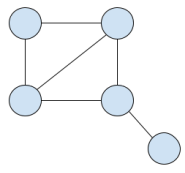
\includegraphics[width=1cm,keepaspectratio]{images/5sujet} \\
            \midrule
            
\includegraphics[width=1cm,keepaspectratio]{images/1}            & 3                                                            & 4                                                             & 4                                                              & 5                                                          \\
            
\includegraphics[width=1cm,keepaspectratio]{images/2}            & 3                                                            & 4                                                             & 4                                                              & 6                                                          \\
            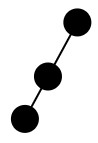
\includegraphics[width=1cm,keepaspectratio]{images/3}            & 3                                                            & 5                                                             & 2                                                              & 10                                                         \\
            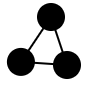
\includegraphics[width=1cm,keepaspectratio]{images/3tr}          & 1                                                            & 1                                                             & 0                                                              & 2                                                          \\
            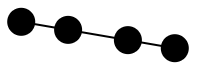
\includegraphics[width=1cm,height=1cm,keepaspectratio]{images/4} & 0                                                            & 1                                                             & 1                                                              & 10                                                         \\
            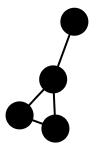
\includegraphics[width=1cm,keepaspectratio]{images/4tr}          & 0                                                            & 1                                                             & 0                                                              & 5                                                          \\
            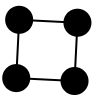
\includegraphics[width=1cm,keepaspectratio]{images/4carre}       & 0                                                            & 0                                                             & 0                                                              & 1                                                          \\
            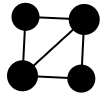
\includegraphics[width=1cm,keepaspectratio]{images/4carBarre}    & 0                                                            & 0                                                             & 0                                                              & 1                                                          \\
            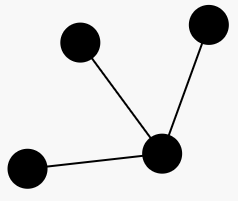
\includegraphics[width=1cm,keepaspectratio]{images/4trois+}      & 0                                                            & 1                                                             & 0                                                              & 4                                                          \\
            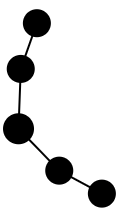
\includegraphics[width=1cm,keepaspectratio]{images/5}            & 0                                                            & 0                                                             & 0                                                              & 4                                                          \\
            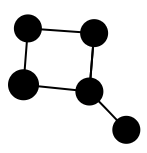
\includegraphics[width=1cm,keepaspectratio]{images/5Carr}        & 0                                                            & 0                                                             & 0                                                              & 1                                                          \\
            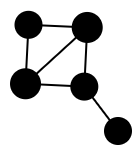
\includegraphics[width=1cm,keepaspectratio]{images/5CarrBare}    & 0                                                            & 0                                                             & 0                                                              & 1                                                          \\
            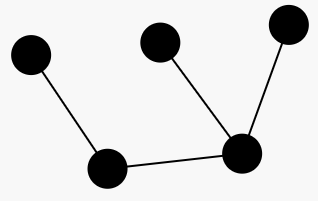
\includegraphics[width=1cm,keepaspectratio]{images/5quatre+}     & 0                                                            & 0                                                             & 0                                                              & 4                                                          \\
            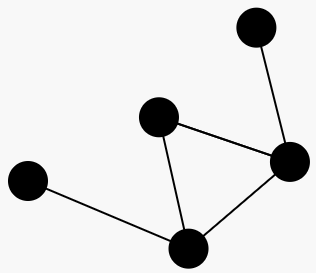
\includegraphics[width=1cm,keepaspectratio]{images/5+tr+}        & 0                                                            & 0                                                             & 0                                                              & 2                                                          \\
            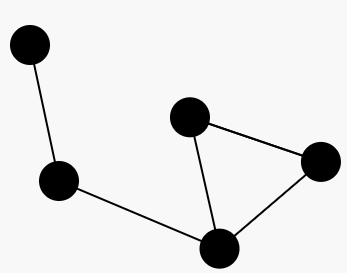
\includegraphics[width=1cm,keepaspectratio]{images/5Tr++}        & 0                                                            & 0                                                             & 0                                                              & 2                                                          \\
            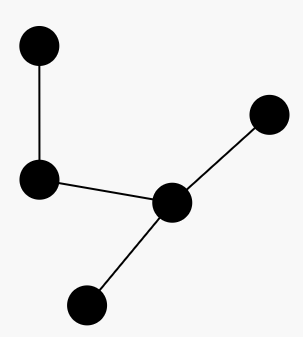
\includegraphics[width=1cm,keepaspectratio]{images/5trois+deux}  & 0                                                            & 0                                                             & 0                                                              & 2                                                          \\
            \bottomrule
        \end{tabular}
        \caption{Feature Values}
    \end{table}

\end{document}
